\documentclass{article}
\usepackage[utf8]{inputenc}
\usepackage[spanish]{babel}
\usepackage{amsmath}
\usepackage{amssymb}
\usepackage{amsfonts}
\usepackage{hyperref}
\usepackage{textcomp}
\usepackage{graphicx}
\usepackage{pgfplots}
\usepackage{geometry}
\hypersetup{
    colorlinks=true,
    linkcolor=black,
    citecolor=green,
    filecolor=magenta,      
    urlcolor=cyan,
}
\geometry{
  top=3cm,            % Margen superior
  bottom=3cm,         % Margen inferior
  left=3cm,           % Margen izquierdo
  right=3cm           % Margen derecho
}

\title{Estadística 1}
\author{Jorge Miguel Alvarado Reyes}
\date{16 Agosto 2023}

\setlength{\parindent}{0pt}
\begin{document}

\begin{titlepage}
    \begin{center}
        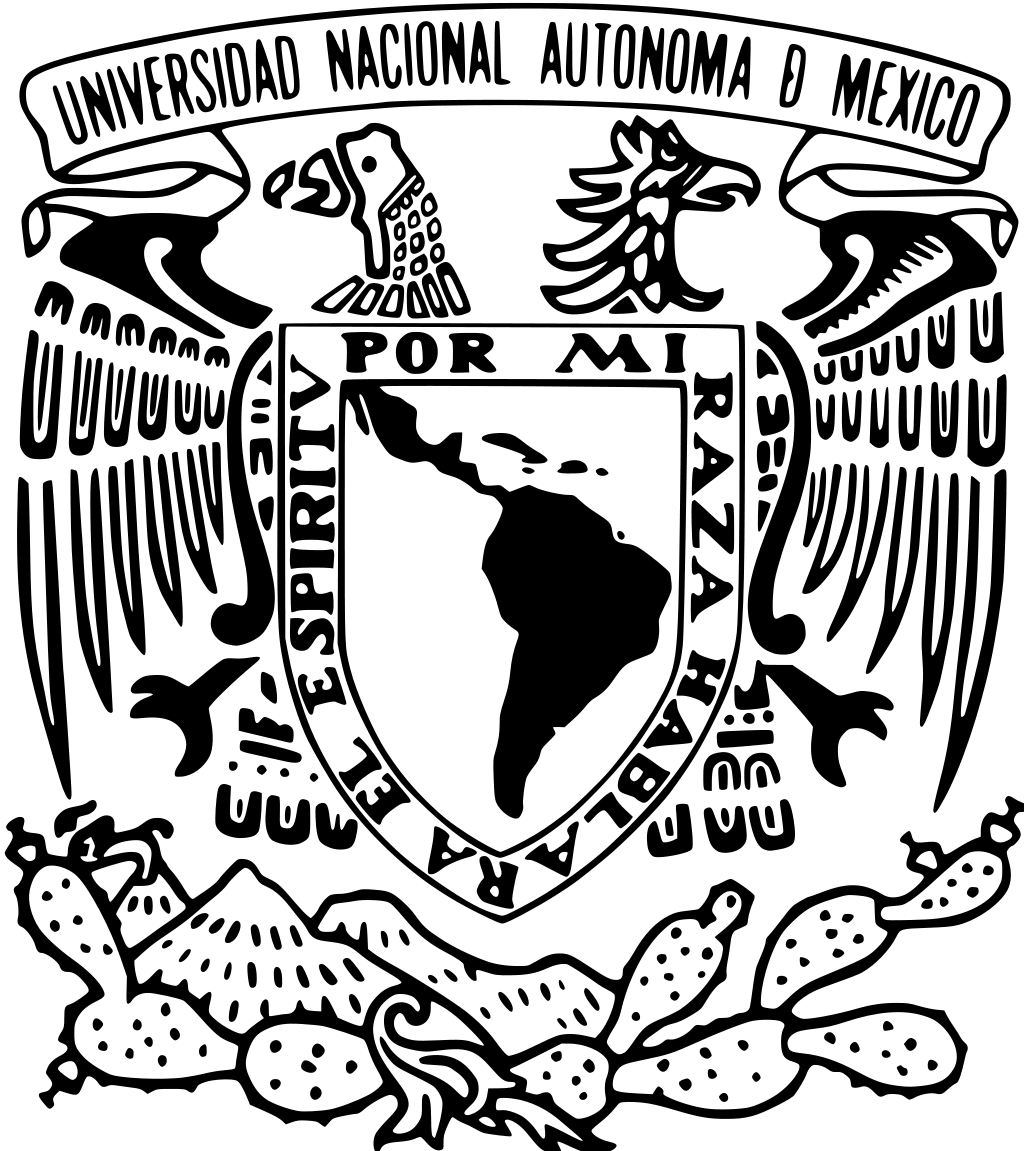
\includegraphics[width=0.2\textwidth]{../../unam.png}
        \vspace*{.5cm}

        \LARGE
        \textbf{Universidad Nacional Autónoma de México}

        \vspace{0.5cm}
        \LARGE
        Facultad de Estudios Superiores Acatlán

        \vspace{2cm}

        \textbf{Examen Unidad 1} \\
        Ecuaciones Diferenciales

        \vfill

        \vspace{1cm}

        \textbf{\large Autor:} \\
        Jorge Miguel Alvarado Reyes \\
        421010301\\
        \vspace{.5cm}
        \normalsize \today

    \end{center}
\end{titlepage}
\newpage

\tableofcontents

\newpage

\section{3}
Observe entonces que
\[
\mathcal{L}^{-1}\{F(s)G(s)\} = \int_0^{\infty} f(\tau)g(t - \tau) \, d\tau,
\]
determine la Transformada Inversa de Laplace de


\subsection{3.4}
\[
    F(s) = \frac{7s^2+7s-14}{s^6+3s^4+3s^2+1}, \quad G(s) = \frac{2}{s^2}
\]

\section{4}
Encuentre la solución de las siguientes ecuaciones diferenciales.

\subsection{4.1}

\[
    y''(t) + 2y'(t) + 2y(t) = \delta(t-5), \quad y(0)=1, \quad y'(0)=0
\]
\subsection{4.2}

\[
    y''(t) + 4y'(t) + 3y(t) = 1 + \delta(t-3), y(0)=0, y'(0) = 1
\]
\end{document}